\section{Simulation Framework} 
\label{sec:framework}
We leverage an existing open-source HLS framework called LegUp \cite{canis2013legup} that takes a C program as input and outputs a hardware RTL design. 
In \cite{huang2013effect}, an approach is devised to quickly determine the number of hardware execution cycles without requiring time-consuming logic simulation.
We develop our reinforcement learning simulator environment based on the existing harness provided by LegUp and  validate our final results by going through the time-consuming logic simulation. The framework takes a program (or multiple programs) and intelligently explores the space of possible passes to figure out an optimal pass sequence to apply. The framework is illustrated in Figure~\ref{fig:framework}.

\subsection{HLS Compiler}
Our framework takes a set of programs as input and compiles them using the Clang front-end of the LLVM compiler. LLVM represents programs in a hardware-independent intermediate representation (IR). Optimization and analysis passes act as transformations on the IR, taking a program as input and emitting a new IR as output. The HLS tool LegUp is invoked after the compiler optimization as a back-end pass, which transforms LLVM IR into hardware modules.
%The compute logic is turned into a hardware datapath and the control logic is turned into a hardware FSM respectively by the HLS tool. 
%Its SDC-based scheduler \cite{cong2006efficient} operates at the basic block level to exploit the instruction-level parallelism. 

\subsection{Clock-cycle Time Profiler}
Once the hardware RTL is generated one could run a hardware simulation to gather the cycle count results of the synthesized circuit. This process is quite time-consuming, hindering RL and all other optimization approaches. Therefore, we approximate cycle count using the profiler in LegUp~\cite{huang2013effect}, which runs $20\times$ faster than hardware simulation. 
In LegUp, the frequency of the generated circuits is set as a compiler constraint that directs the HLS scheduling algorithm. In other words, HLS tool will always try to generate hardware that can run at a certain frequency. In our experiment setting, without loss of generality, we set the target frequency of all generated hardware to 50MHz.
%The profiler first runs the software program to gather information on the number of times each basic block is executed, then multiplies it with the clock cycle time of the basic block determined by the HLS scheduler to produce the total clock cycle time of the circuit. This software approach is $20\times$ faster than hardware simulation, which significantly reduces the runtime bottleneck of the deep reinforcement learning algorithm. 

\subsection{IR Feature Extractor}
In addition to the LegUp backend tools, we developed analysis passes to extract 56 static features from the program, such as the number of basic blocks, branches, and instructions of various types. 
%Each individual feature is insufficient to guide the machine learning algorithm.
We use these features as partially observable states for the RL learning and hope the neural network can capture the correlation of certain combination of these features and certain optimization. Unfortunately, due to the page limit, we could not include the table of features. 
%All the features we gather are listed in Table~\ref{tab:tab1} in the appendix. 
%The framework takes a program or multiple ones and compiles them using the LLVM compiler, which was modified to output the program features. The HLS toolchain is used to extract the number of cycles that are used as the cost function to the RL architecture to find the optimal passes. 

\subsection{Deep Reinforcement Learning Framework}
We wrapped compilation utilities into a Python script and wrote an environment simulator with APIs similar to an OpenAI gym~\cite{brockman2016openai}. Our utilities take an input a program (as LLVM IR) and returns the program feature vectors and the total number of clock cycles. We consider two types of features as the state for the RL: the current program IR and the sequence of passes that have been applied. The overall flow works as follows:
\begin{enumerate}
\item The program is compiled into LLVM IR. 
\item LegUp compiles the LLVM IR into hardware RTL and produces an estimated clock-cycle time for the generated circuit. 
\item The IR feature extractor is run to extract program features. 
\item The clock-cycle time and program features are fed into various machine learning algorithms (random, genetic, greedy, and RL) to derive a good LLVM optimization sequence. In RL specifically, the clock-cycle time is used for reward calculation, and the program features are used as partially observable states for the RL agents. 
\item In iterative methods (\textit{i.e.}, greedy algorithm, genetic algorithm, and RL), the algorithm then predicts the next best action to take. In RL, the action would be the next optimization to apply to the end of an existing sequence of passes. In a modified greedy algorithm, the next action could be the next best place to insert the optimization pass.
\item New LLVM IR is generated after the new optimization sequence is applied. 
\item The machine learning algorithm iterates through steps 2)--6) until convergence.
\end{enumerate}


\begin{figure}[h!]
    \centering
    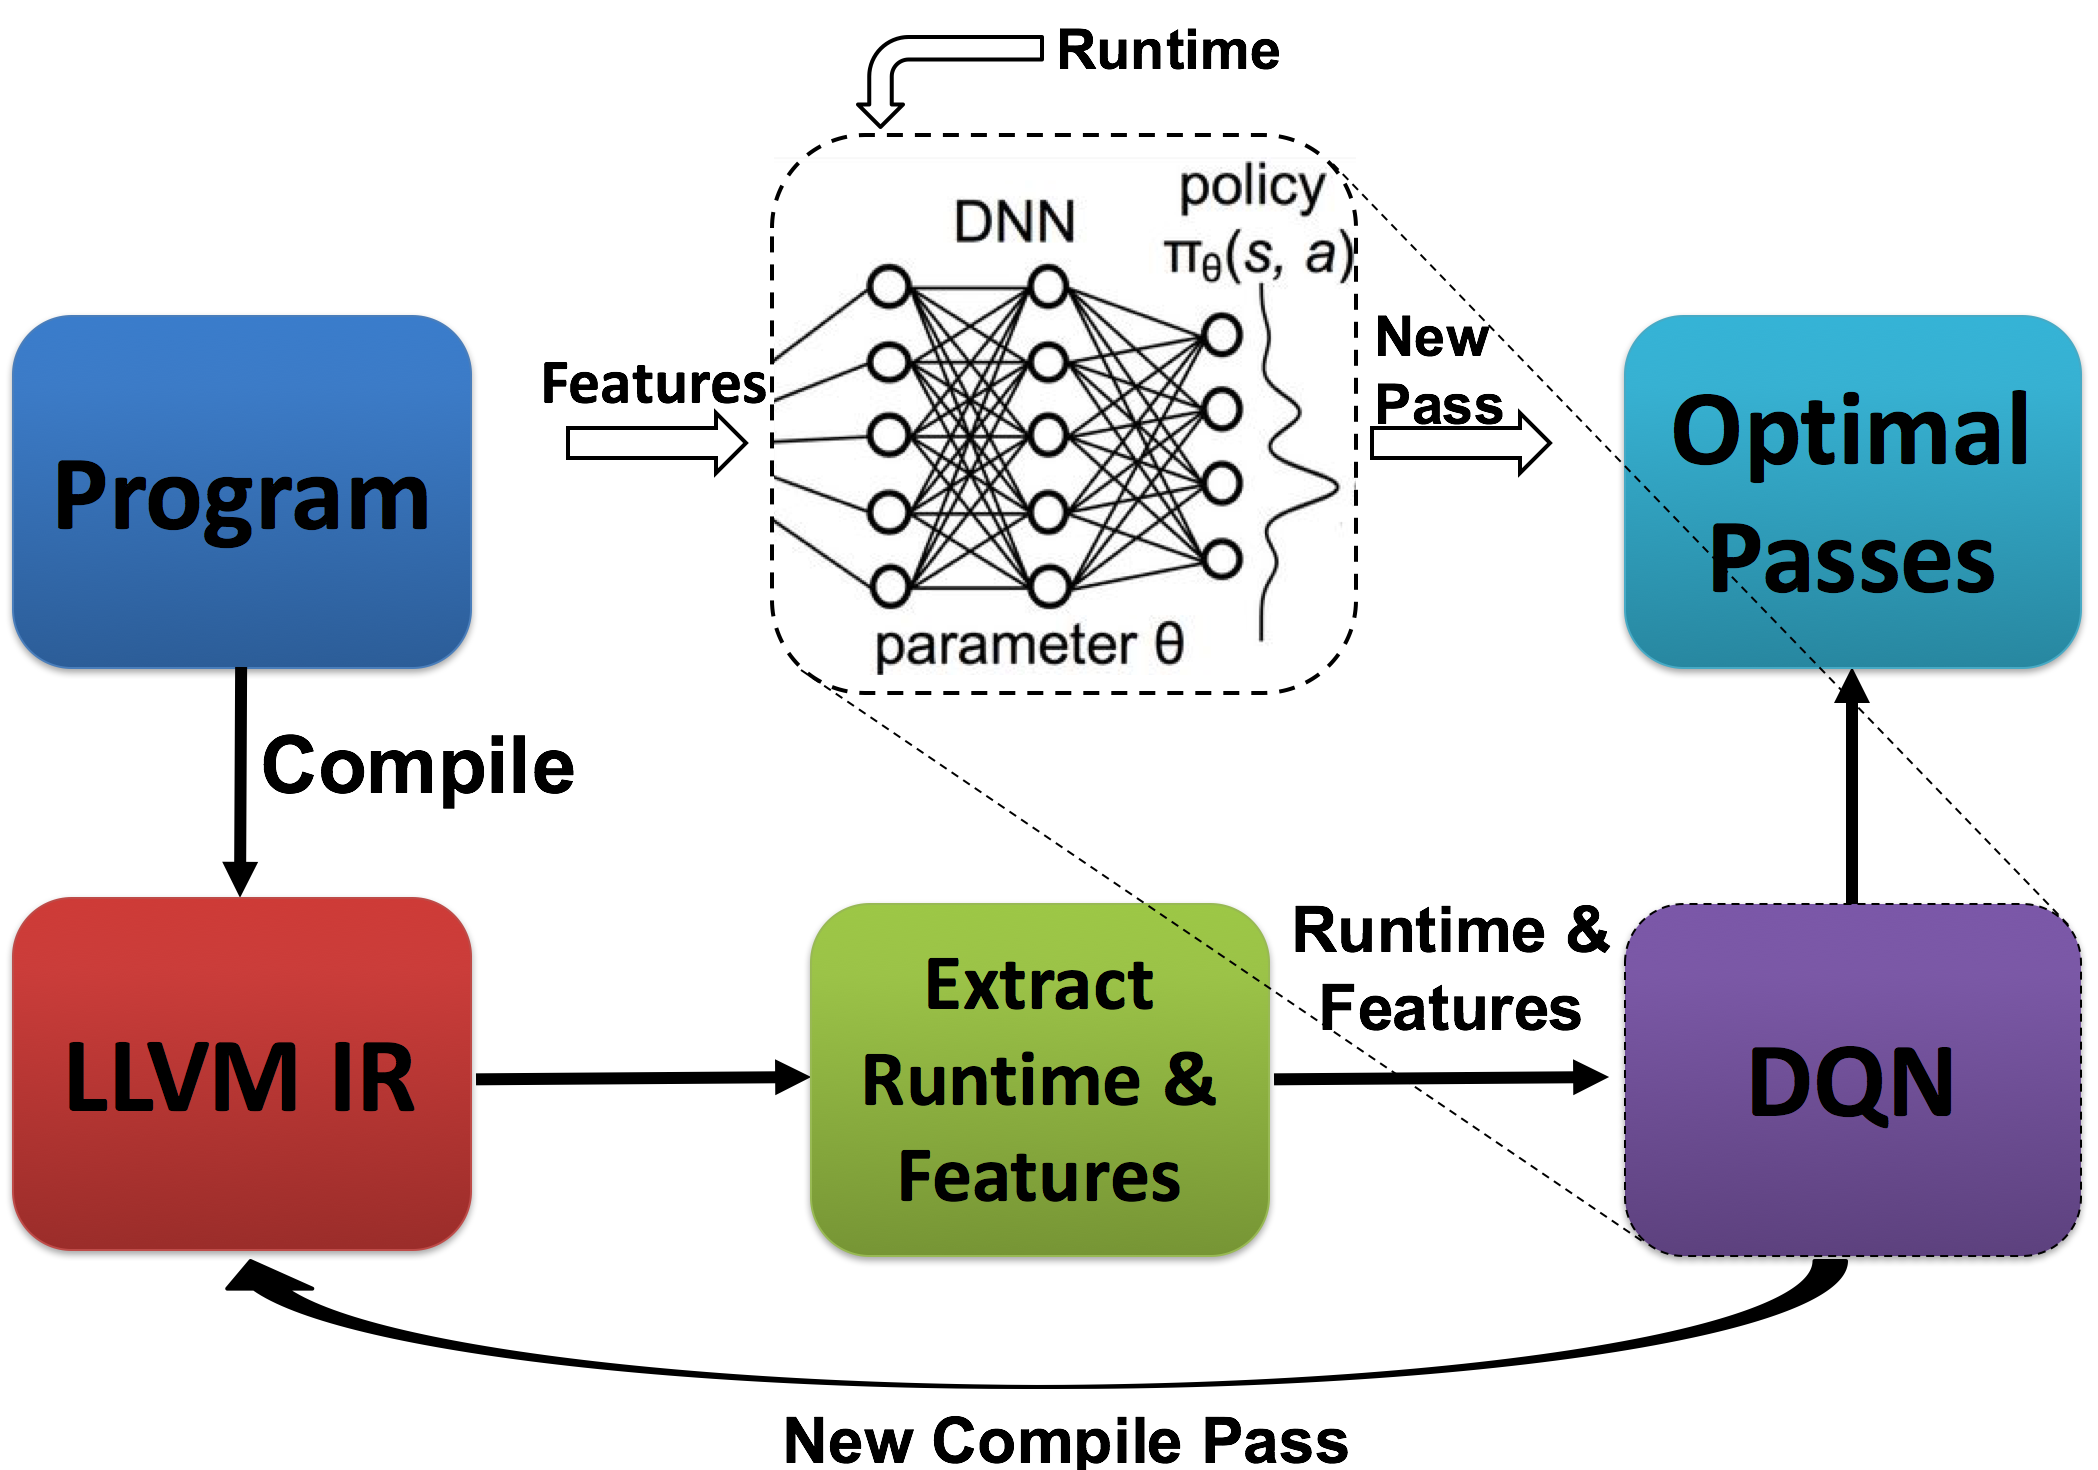
\includegraphics[width=0.5\textwidth]{Figures/framework.png}
    \caption{A block diagram of our framework. The programs are compiled using the Clang/LLVM, features and cycles are extracted from the IR and HLS toolchain respectively, and are afterwards fed to the RL network that tries to learn the optimal passes.  \vspace*{-0.5cm}}
    \label{fig:framework}
\end{figure}
